\documentclass[12pt,a4paper]{scrartcl}
\usepackage[utf8]{inputenc}
\usepackage[english,russian]{babel}
\usepackage{amssymb,amsfonts}
\usepackage{amsmath,cite,enumerate}
\usepackage{float,indentfirst}
\usepackage{graphicx}
\usepackage{geometry} % Меняем поля страницы
\geometry{left=2cm}% левое поле
\geometry{right=1.5cm}% правое поле
\geometry{top=1cm}% верхнее поле
\geometry{bottom=2cm}% нижнее поле
\graphicspath{{images/}}

\begin{document}


\begin{titlepage}
  \begin{center}
    Санкт-Петербургский Политехнический Университет     Петра Великого \\
    
    Институт компьютерных наук и технологий \\
    
    Кафедра компьютерных систем и программных технологий
  \end{center}
  
  \vfill
  
  \begin{center}
  Лабораторная работа №3\\
  по теме\\
  "Сигналы телекоммуникационных
систем"\\
\end{center}

\vfill

\newlength{\ML}
\settowidth{\ML}{«\underline{\hspace{0.7cm}}» \underline{\hspace{2cm}}}
\hfill\begin{minipage}{0.4\textwidth}
  Выполнил студент группы 33501/3\\
  \underline{\hspace{\ML}} Кисличенко Б.\,Д\\
\end{minipage}%

\bigskip

\settowidth{\ML}{«\underline{\hspace{0.7cm}}» \underline{\hspace{2cm}}}
\hfill\begin{minipage}{0.4\textwidth}
  Руководитель\\
  \underline{\hspace{\ML}} Богач Н.\,В\\
\end{minipage}%

\vfill
 
\begin{center}
  Санкт-Петербург\\
2018 
\end{center}

\end{titlepage}

\section{Цель}
\label{sec:goal}

Изучить воздействие ФНЧ на тестовый сигнал с шумом.\\

\section{Постановка задачи}
\label{sec:task}

Сгенерировать гармонический сигнал с шумом и синтезировать ФНЧ. Получить сигнал во временной и частотной областях до и после фильтрации. Сделать выводы о воздействии ФНЧ на спектр сигнала.\\

\section{Фильтры}
\label{sec:teoriya}

Одной из часто возникающих на практике задач является создание фильтров,
пропускающих сигналы в определенной полосе частот и задерживающих остальные
частоты. При этом различают:

1) фильтры нижних частот (ФНЧ; английский термин - low-pass filter), пропускающие
частоты, меньшие некоторой частоты среза $\omega 0$;

2) фильтры верхиих частот (ФВЧ; английский термин - l1igh-pass filter), пропускающие
частоты, большие некоторой частоты среза $\omega 0$;

3) полосовые фильтры (ПФ; английский термин - band-pass filter), пропускающие
частоты в некотором диапазоне $\omega 1$ ... $\omega 2$ ( они могут также характеризоваться
средней частотой $\omega 0 = (\omega 1 + \omega 2)/ 2 $ и шириной полосы пропускания $\delta \omega = \omega 2 - \ omega 1);$

4) режекторные фильтры (другие возможные названия - заграждающий фильтр,
фильтр-пробка, полосно-задерживающий фильтр; английский термин - bandstop
filter), пропускающие на выход все частоты, кроме лежащих в некотором
диапазоне $\omega 1$ ... $\omega 2$ ( они тоже могут характеризоваться средней частотой  $\omega 0 = (\omega 1 + \omega 2)/ 2 $ и шириной полосы задерживания $\delta \omega = \omega 2 - \ omega 1);$

\textbf{Частота среза} - частота, выше или ниже которой мощность выходного сигнала уменьшается по сравнению с мощностью в полосе пропускания.

\textbf{Фильтр с конечной импульсной характеристикой (нерекурсивный фильтр, КИХ-фильтр)} — один из видов электронных фильтров, характерной особенностью которого является ограниченность по времени его импульсной характеристики (с какого-то момента времени она становится точно равной нулю). Знаменатель передаточной функции такого фильтра — некая константа. 

\textbf{Фильтр с бесконечной импульсной характеристикой (рекурсивный фильтр, БИХ-фильтр)} — электронный фильтр, использующий один или более своих выходов в качестве входа, то есть образует обратную связь.Основным свойством таких фильтров является то, что их импульсная переходная характеристика имеет бесконечную длину во временной области, а передаточная функция имеет дробно-рациональный вид. Такие фильтры могут быть как аналоговыми так и цифровыми. 

\newpage

\section{Ход работы}
\label{sec:work}

%Рисунок 2
\begin{figure}[h!]
\center{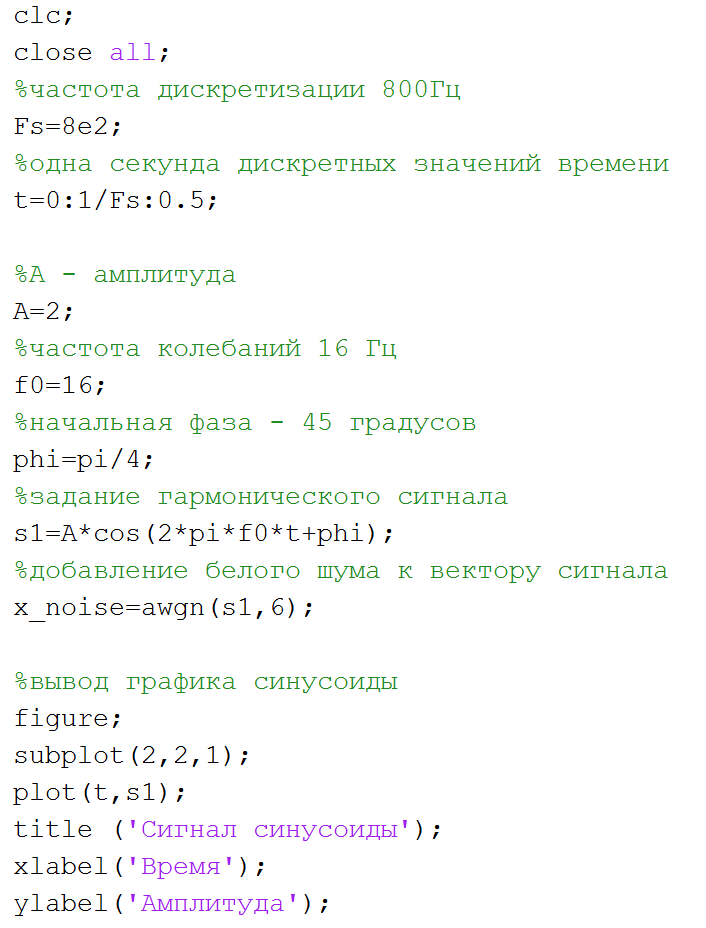
\includegraphics[width=0.9\linewidth]{part1}}
\caption{Генерируем синусоидальный сигнал? добавляем к нему шум и выводим его}
\end{figure}

%Рисунок 3
\begin{figure}[h!]
\center{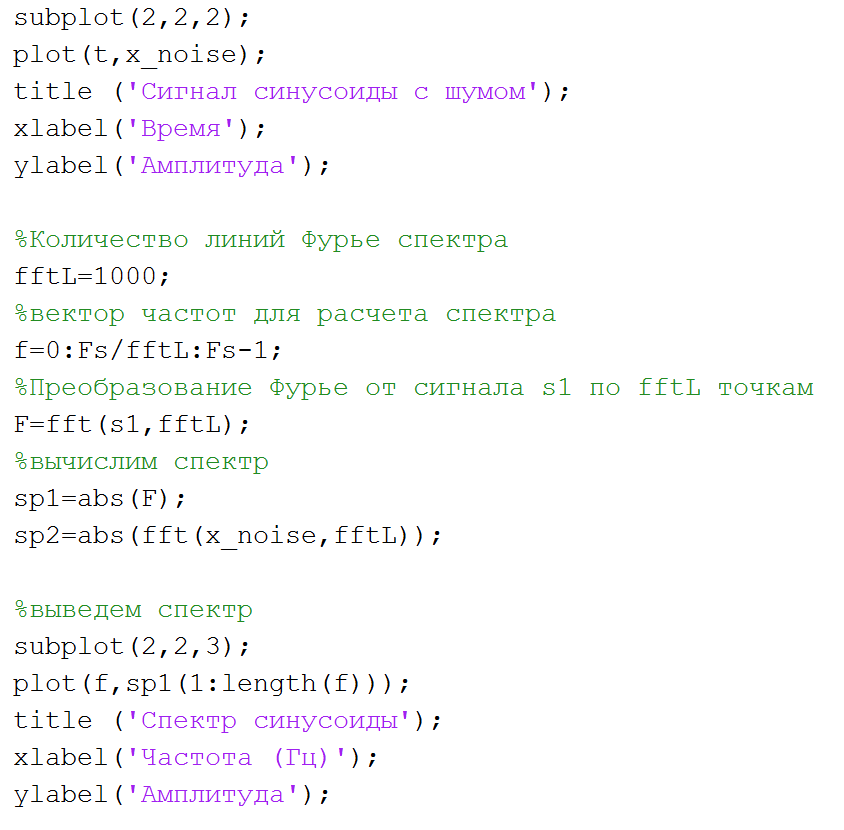
\includegraphics[width=0.9\linewidth]{part2}}
\caption{Получаем спектры синусоидального сигнала и сигнала с шумом}
\end{figure}

%Рисунок 4
\begin{figure}[h!]
\center{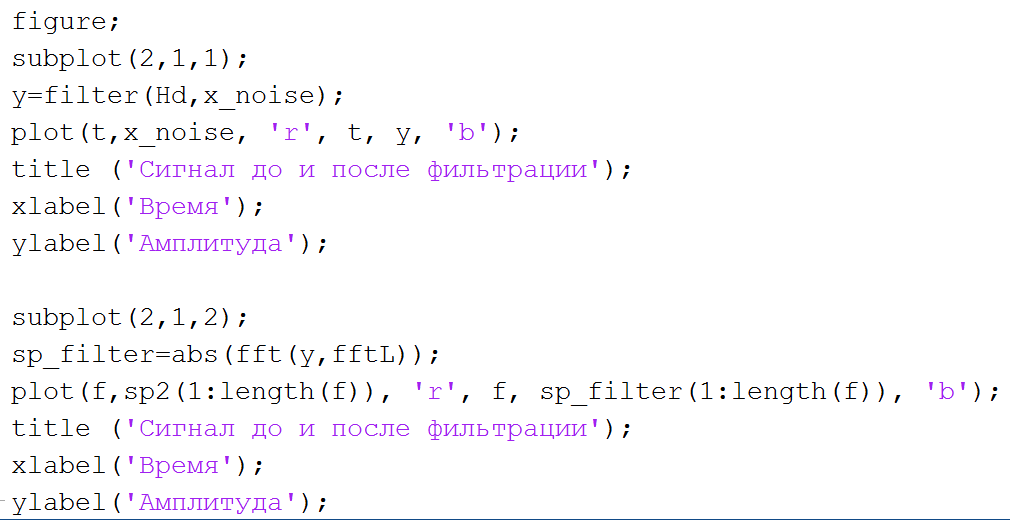
\includegraphics[width=0.9\linewidth]{part3}}
\caption{Применяем фильтр и выводим результат}
\end{figure}
\newpage

%Рисунок 5
\begin{figure}[h!]
\center{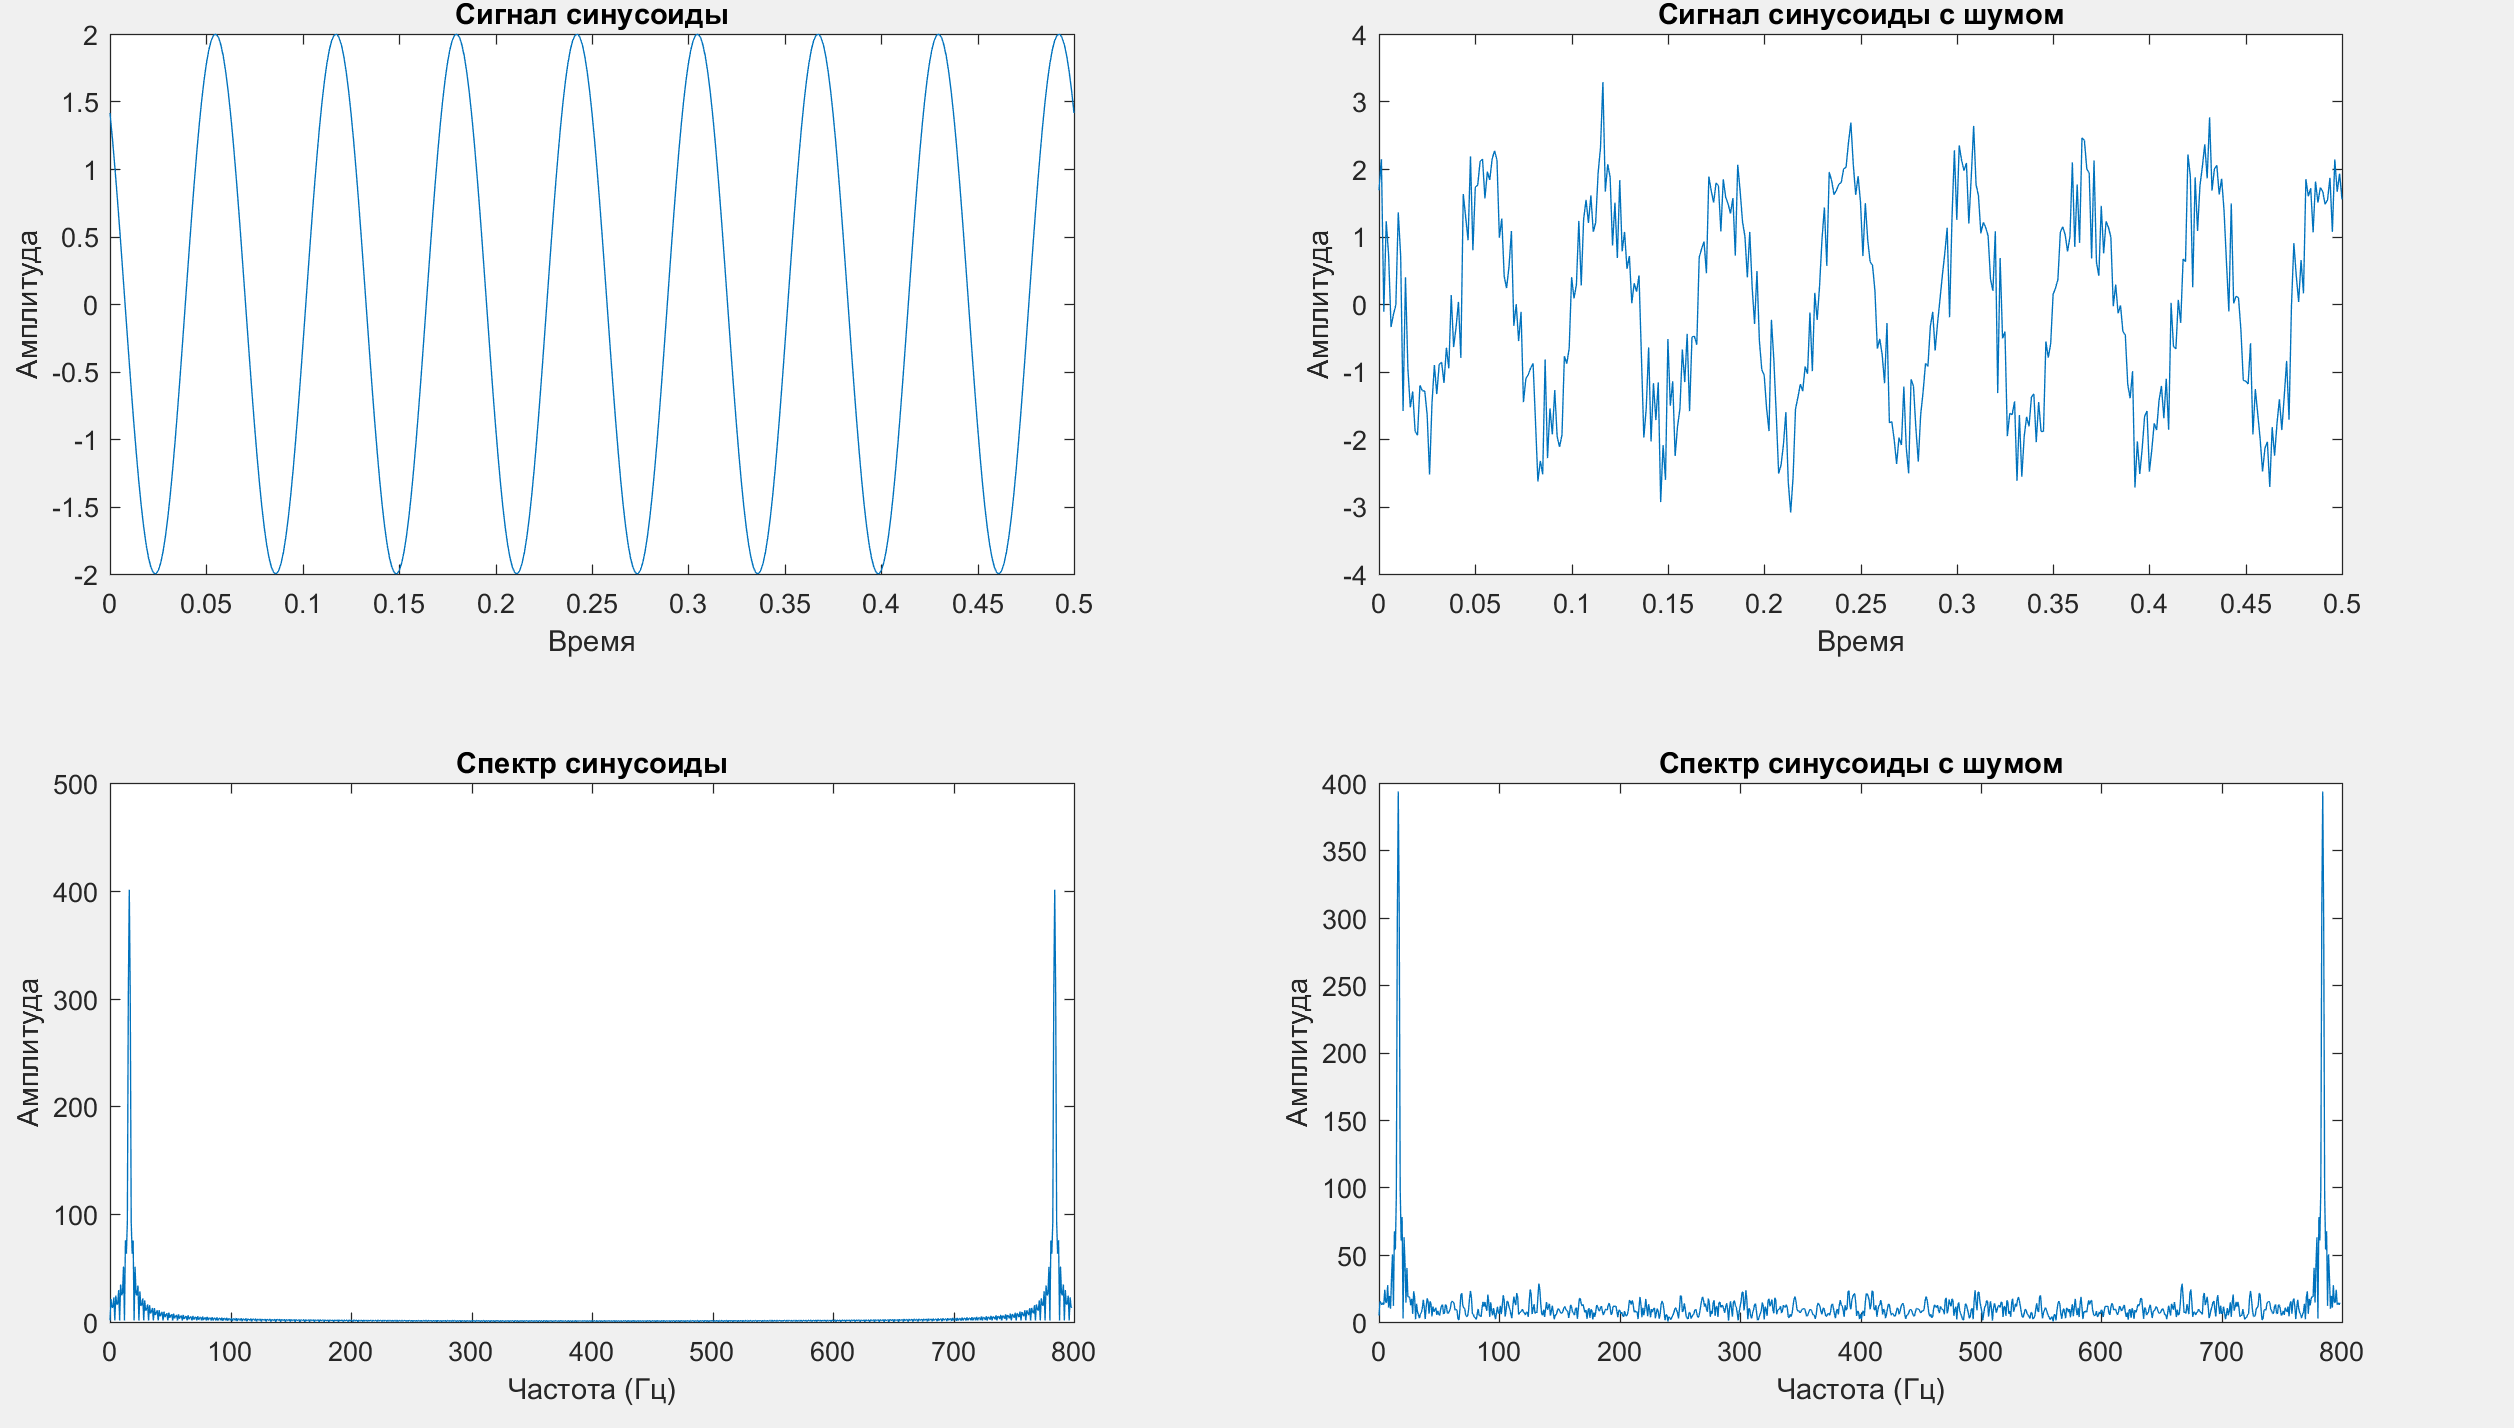
\includegraphics[width=0.9\linewidth]{sin_noise}}
\caption{Синусоида с шумом и без со спектрами}
\end{figure}
\newpage

%Рисунок 6
\begin{figure}[h!]
\center{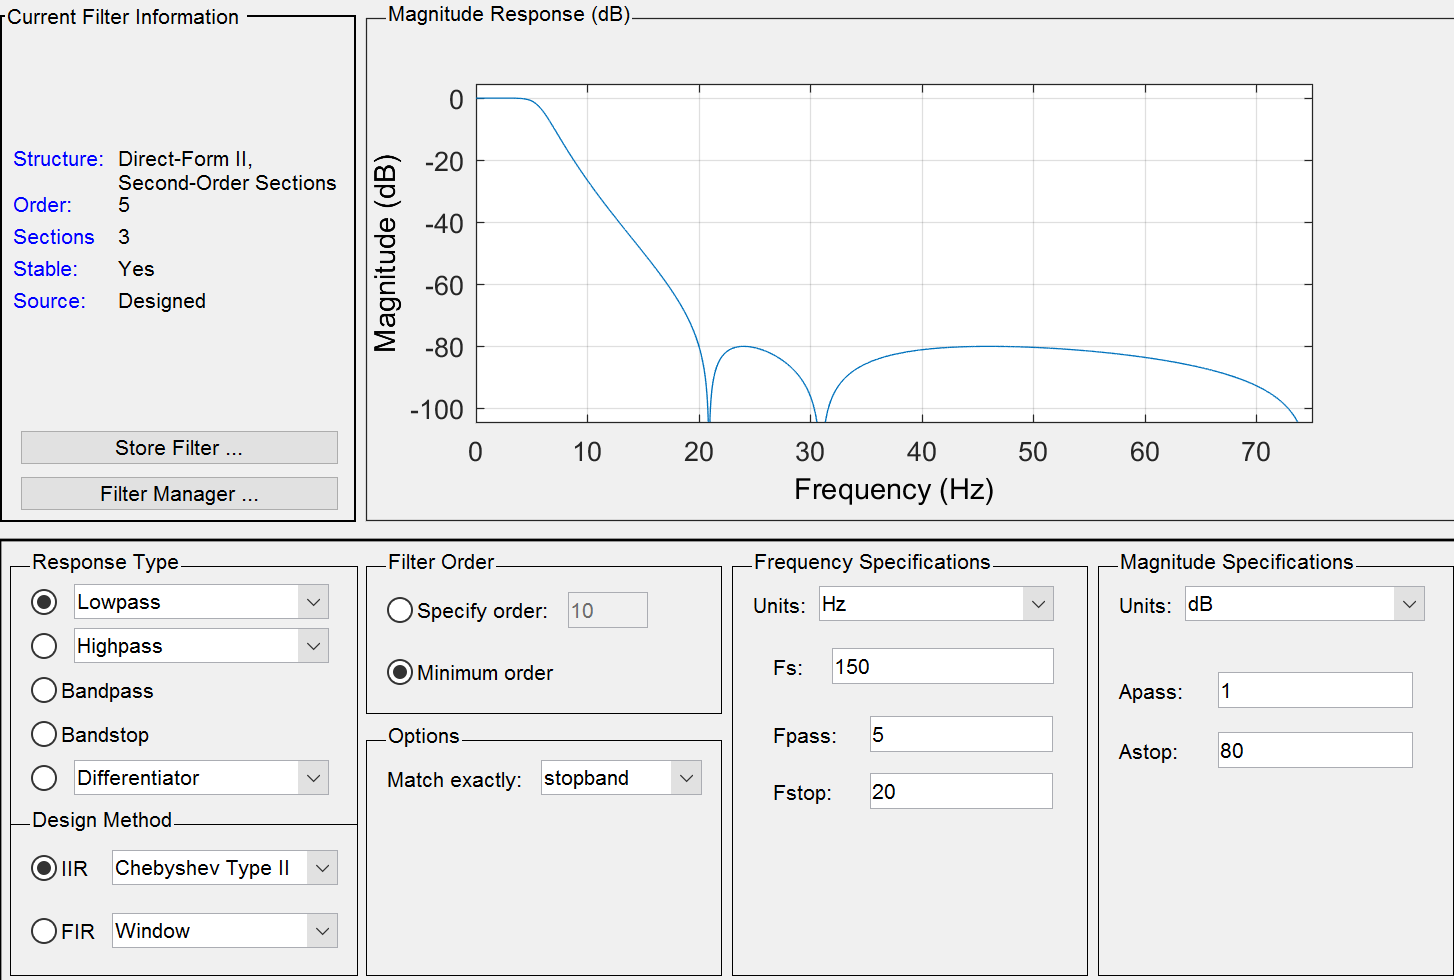
\includegraphics[width=0.9\linewidth]{cheb_2}}
\caption{Настройка рекурсивного фильтра типа chebyshev type II}
\end{figure}
\newpage


%Рисунок 7
\begin{figure}[h!]
\center{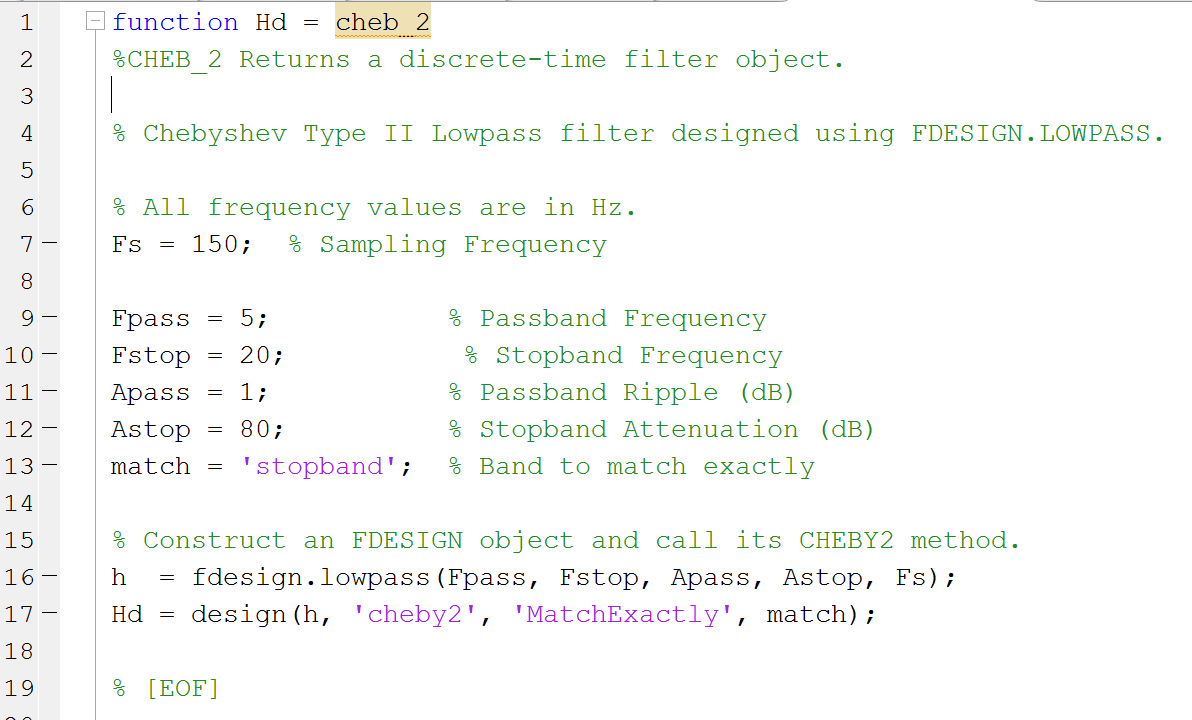
\includegraphics[width=0.9\linewidth]{cheb_2_code}}
\caption{Код фильтра типа chebyshev type II}
\end{figure}

%Рисунок 8
\begin{figure}[h!]
\center{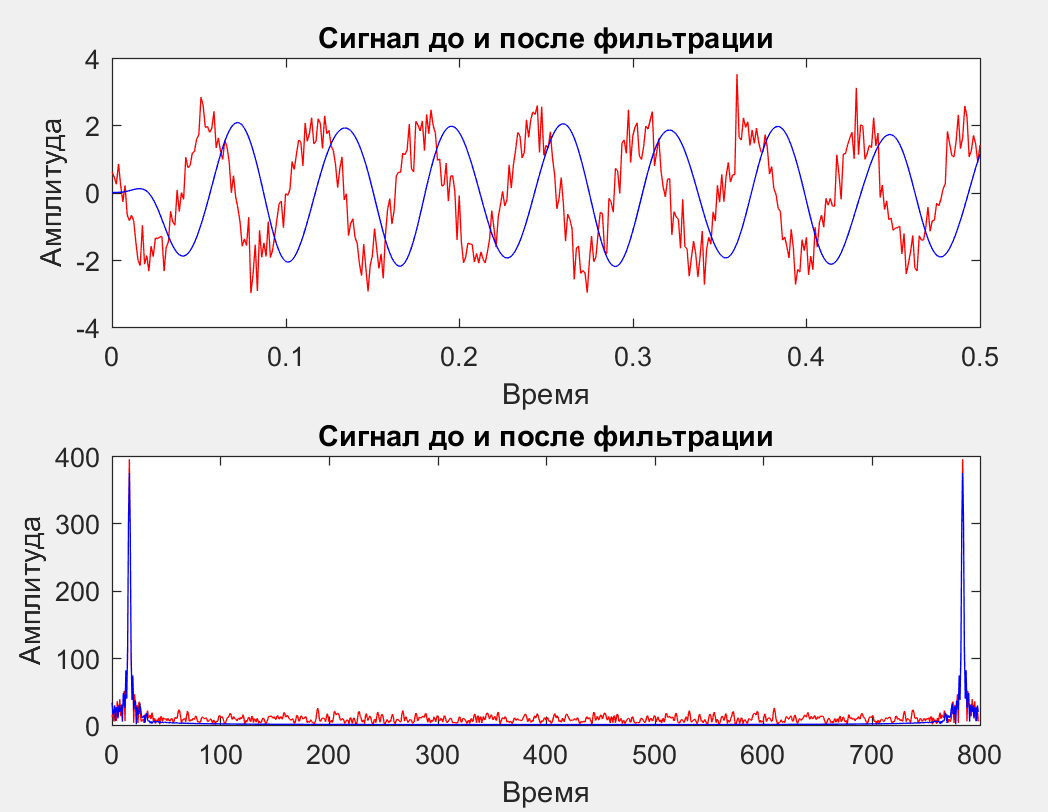
\includegraphics[width=0.9\linewidth]{cheb_2_sp}}
\caption{Отфильтрованный сигнал филтром БИХ и его спектр}
\end{figure}

%Рисунок 9
\begin{figure}[h!]
\center{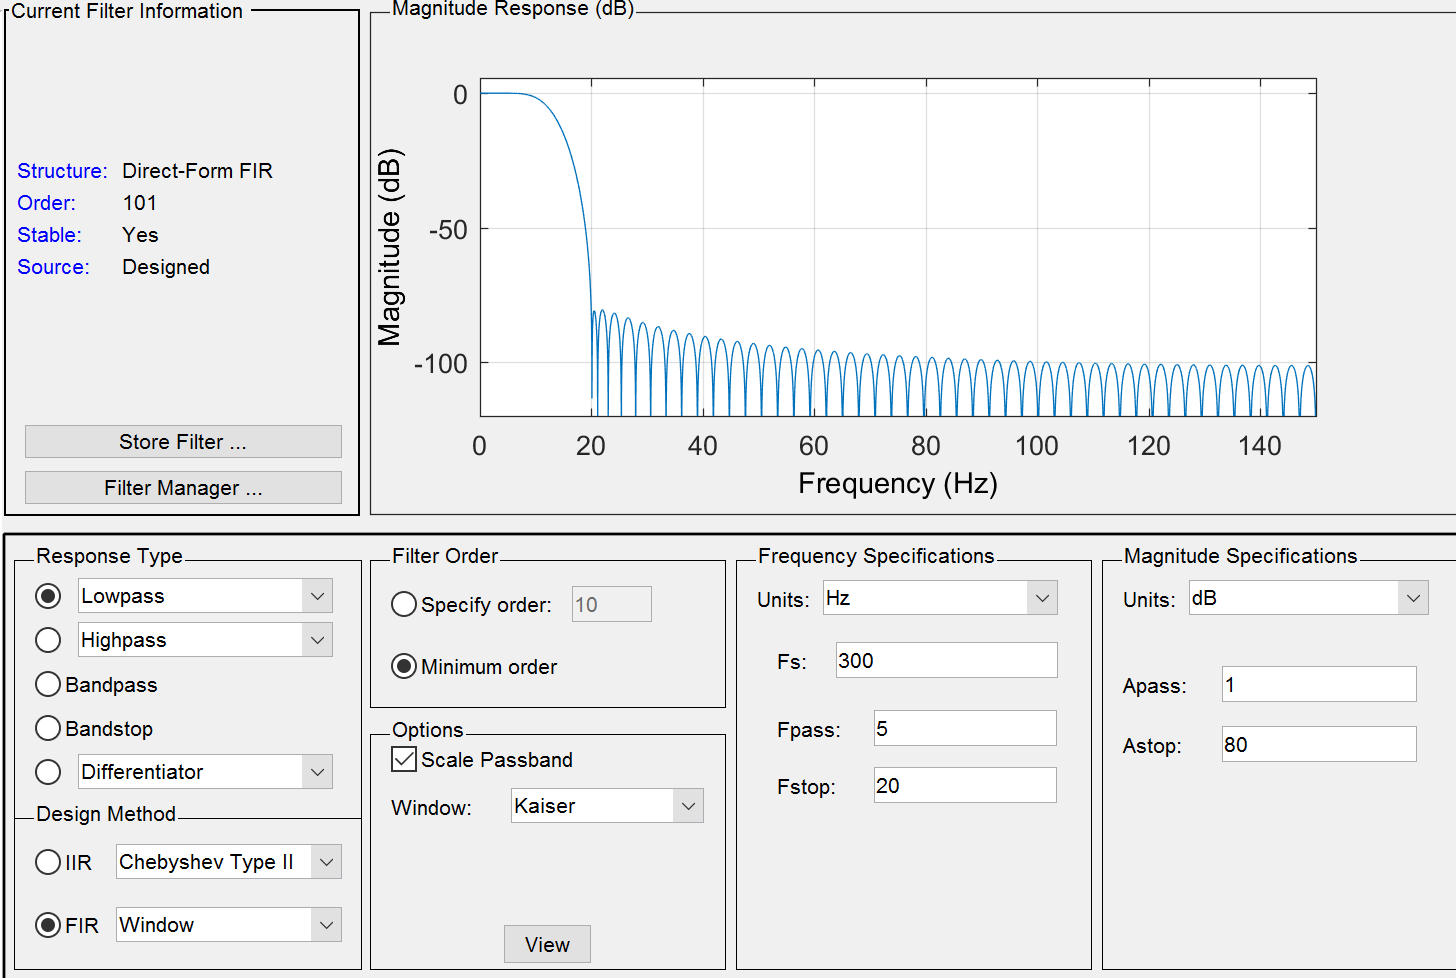
\includegraphics[width=0.9\linewidth]{kaiser}}
\caption{Настройка КИХ фильтра (окно kaiser)}
\end{figure}

%Рисунок 10
\begin{figure}[h!]
\center{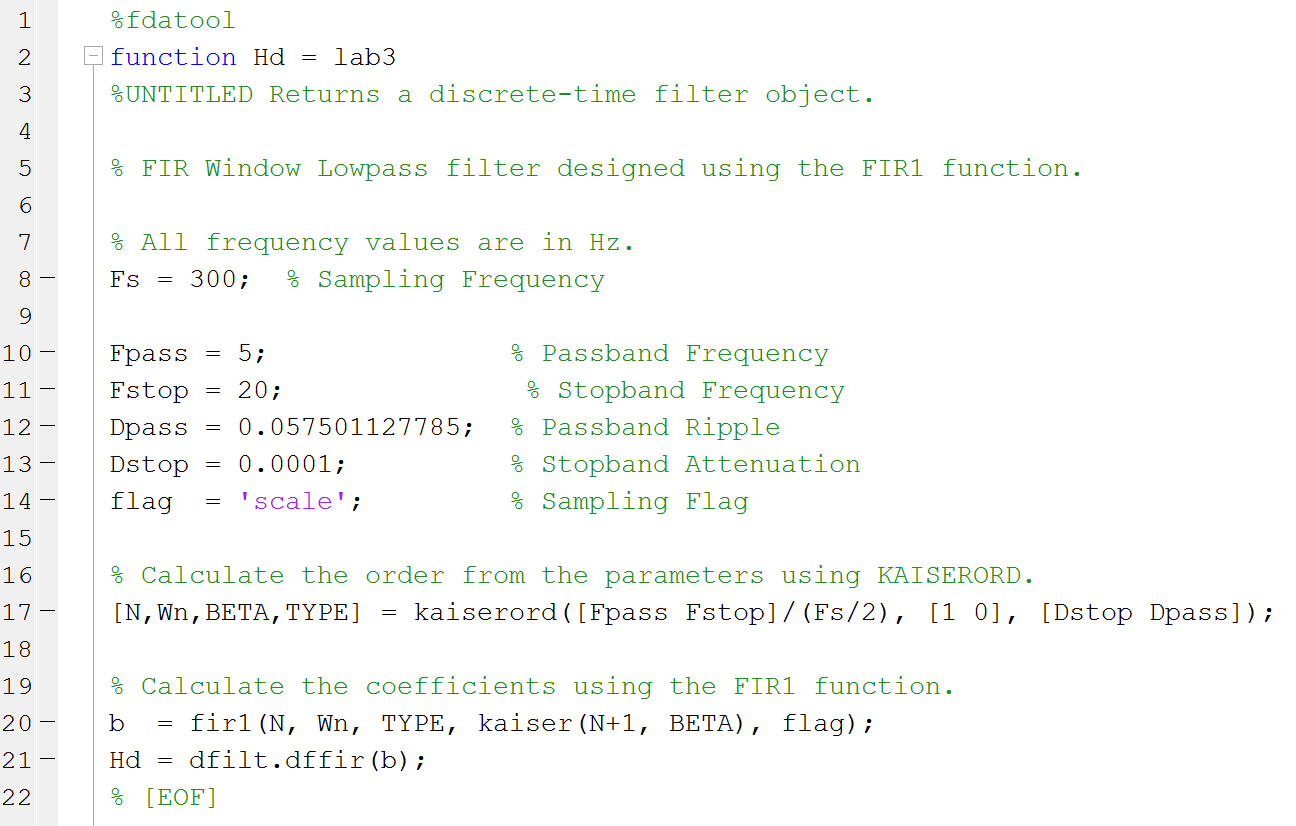
\includegraphics[width=0.9\linewidth]{kaiser_code}}
\caption{Код КИХ фильтра}
\end{figure}

%Рисунок 11
\begin{figure}[h!]
\center{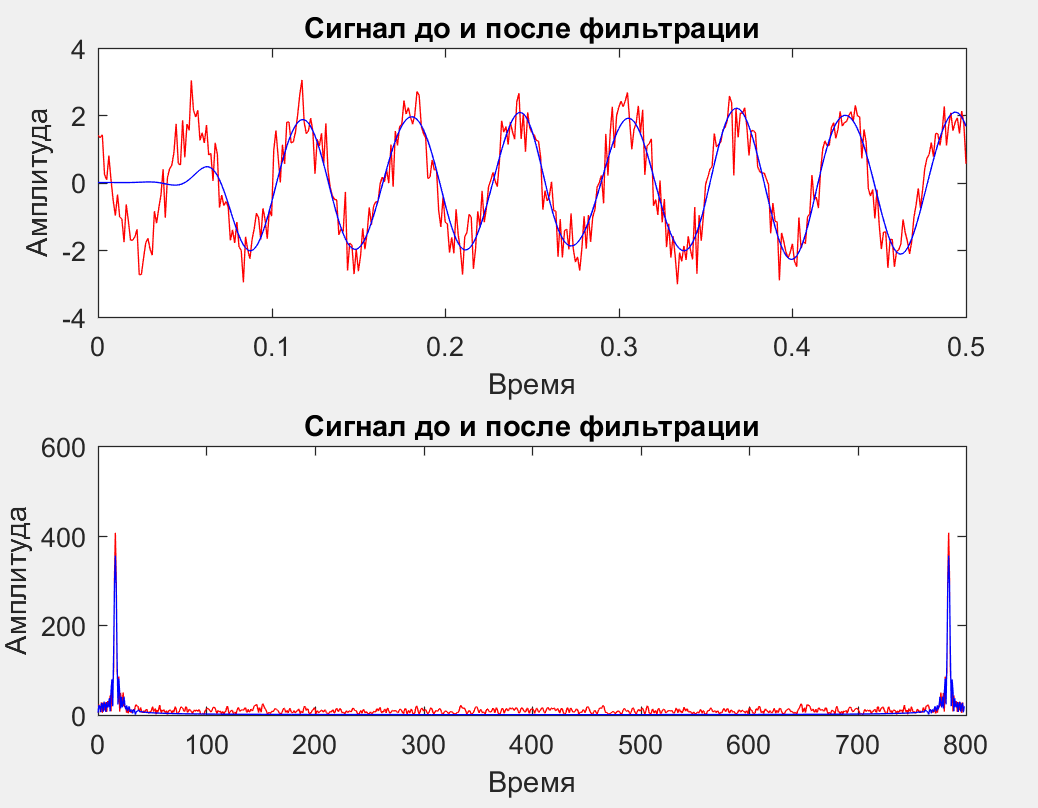
\includegraphics[width=0.9\linewidth]{kaiser_sp}}
\caption{Отфильтрованный сигнал филтром КИХ и его спектр}
\end{figure}

\clearpage
\newpage

\section{Вывод}
\label{sec:afterWork}
В ходе данной лабораторной работы мы познакомились со средствами генерации и описания фильтров. Был сгенерированы ФНЧ двух видов - КИХ и БИХ (фильтр Чебышева второго рода).
После фильтрации был получен сигнал с небольшими искажениями и сдвигом. При этом использование и настройка КИХ фильтра позволило добиться лучшего результата и смещения, чем при использовании БИХ фильтра (см. рис.8 и рис.11).

%Рисунок 12
\begin{figure}[h!]
\center{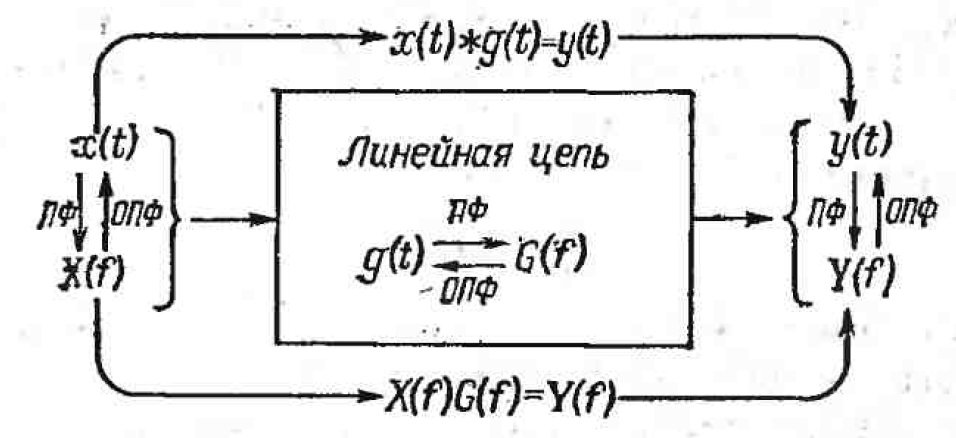
\includegraphics[width=0.9\linewidth]{lin_sig}}
\caption{Преобразование сигнала линейной целью}
\end{figure}

Преобразование дискретных сигналов в линейных цепях описывается в принципе теми же соотношениями, что и преобразования непрерывных сигналов. Отличия заключаются лишь в том, что в случае дискретного сигнала соответсвующий интеграл вырождается в сумму.

Что касается результирующего сигнала, искажения в сигнале остаются из-за неотфильтрованных шумов, который может совпадать с сигналом.


\end{document}